\section{Evaluation}
\label{sec:evaluation}

We evaluate \name{} on two datasets, Waymo and Cityscapes. The main results are:

\begin{itemize}
    \item With multiple cameras sharing the same resources on an edge server, \name{} achieves upto 31.2\% points higher accuracy. Attaining the same accuracy with existing fair scheduling techniques would require upto $4.3\times$ more resources.
    \item With reduced resource provisioning, Ekya's performance gracefully degrades to the basline with no retraining by evaluating the cost of retraining on inference accuracy. 
\end{itemize}

\subsection{Methodology}
\label{subsec:eval-setup}

\noindent\textbf{Datasets.} For our evaluation, we use the Waymo Open\cite{waymo} and Cityscapes\cite{cityscapes} datasets, two popular video datasets containing dashcam footage of cars driving through cities in the US and Europe. Cityscapes has \romilc{xx} video streams (a total of \romilc{xx} hours of videos) while Waymo Open has \romilc{xx} video streams (a total of \romilc{xx} hours of videos)

The workload in cityscapes is constructed by treating each city's video as an independent video stream feeding into Ekya for inference and retraining. The workload in Waymo Open is constructed by creating video streams by concatenating segments from the dataset \romil{Zhengxu can add more here}. These workloads are representative of independent video-streams with local variations which necessitate retraining for their specific data-distributions.

\noindent\textbf{Trace driven simulator.}
To evaluate Ekya, we built a simulator to emulates the execution of training and inference jobs under varying resource constraints by collecting traces of accuracy-resource profiles of different configurations offline. This simulator allows custom scheduling policies to be plugged in and modify the run order and resource allocation for different jobs.
% Talk about the assumptions - inference accuracy min GPU, linear scaling etc

\textbf{Hyperparameters.}
For each training job, we create a fixed set of configurations by varying the following hyperparameters - \romilc{List and describe what each of them is.}. Combinations of these hyperparameters are carefully chosen to create a rich diversity in the resource-accuracy profiles of the configurations. 

\textbf{Baselines.}
We compare against two baselines. First is \textit{No-retraining}, which does not ever retrain the model and thus allocates resources only to inference. Second is \textit{Fair Scheduler}\cite{fairsched} which allocates equal resources to all video streams and within a video stream, allocates equal resources to both, training and inference.
% Why are these good baselines?

\textbf{Metrics.}
Our most used metric is Inference Accuracy over time, as described in \S\ref{subsec:formulation}. We also use the number of GPUs provisioned at the edge server as a measure of cost.

\subsection{End-to-end improvement}
\label{subsec:e2e-improvement}

In this section, we evaluate the end-to-end performance of \name{} on our trace simulator. For each of the Waymo and Cityscapes datasets, we run 10 video streams concurrently on Ekya through 5 retraining windows. Each window is 100 seconds long.

Figure \ref{fig:scalability-gpus} compares the performance of \name{} with the baselines when different different quantities of resources are provisioned at the edge server. Compared to the fair scheduler, \name{} achieves upto $17.8\%$ points higher accuracy on the Cityscapes dataset and upto $31.2\%$ \romil{This is the max() number} points higher accuracy on the Waymo dataset. 

While the percentage point gap between \name{} and the fair scheduler baseline decreases as more GPUs are provisioned, the marginal resource-cost of every percentage point increases as the accuracy increases. Table \ref{tab:resource-savings} demonstrates the resource cost of achieving a fixed accuracy across different video streams. A fair scheduler requires upto $4.3\times$ GPUs compared to \name{} to get the same accuracy and this is a best-case estimate, assuming linear scaling of training throughput with GPUs allocated.
% Formulate this as resource saving

% Per city
At a macro level, \name{} ensures that each video stream is strictly better off than not retraining despite non-uniform resource allocation. Figure \ref{fig:multicam-cities} shows the mean inference accuracy for each video stream. \name{} outperforms both baselines, fair allocation and no-retrain. All video streams do not benefit proportionally from retraining - the \name{} profiler is cognizant of this fact and prioritizes resource allocation for video streams which promise a higher accuracy.

%TODO: Add multi camera results - Model this as throughput - how many streams you can support to get the same accuracy.
\romil{TODO: Varying num of cameras}

% Time series - this seems like a very specific example - remove if unnecessary; Show an example where different resources are allocated
Further, Figure \ref{fig:multicam-timeseries} compares the inference accuracy of the V3 video stream from the Cityscapes dataset when 4 GPUs are provisioned. At training tasks 1, 3 and 4, retraining with a fair scheduler results in similar or lower accuracies compared to not retraining. However, \name{} is able to retrain the model and boost the inference accuracy without any degradation. 



% \begin{figure}[h!]
% 	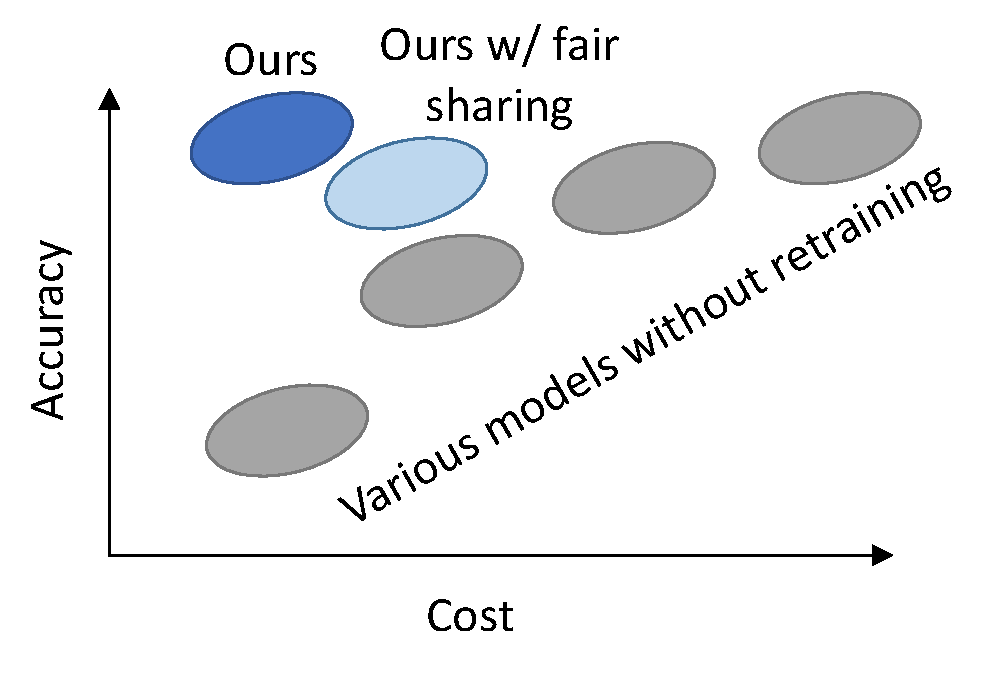
\includegraphics[width=0.4\textwidth]{figures/eval_placeholders/sharing-tradeoffs.pdf}
% 	\caption{\small \bf Multiple video streams sharing an edge cluster: Ours (with adaptive sharing) vs. ours (with fair sharing) vs. various baseline DNNs (without retraining). Our adaptive resource sharing scheme outperforms fair sharing because it is aware of the heterogeneous utility of resource to improve accuracy by different video streams.}
% 	\label{fig:sharing-tradeoffs}
% \end{figure}

% \begin{figure}[h!]
% 	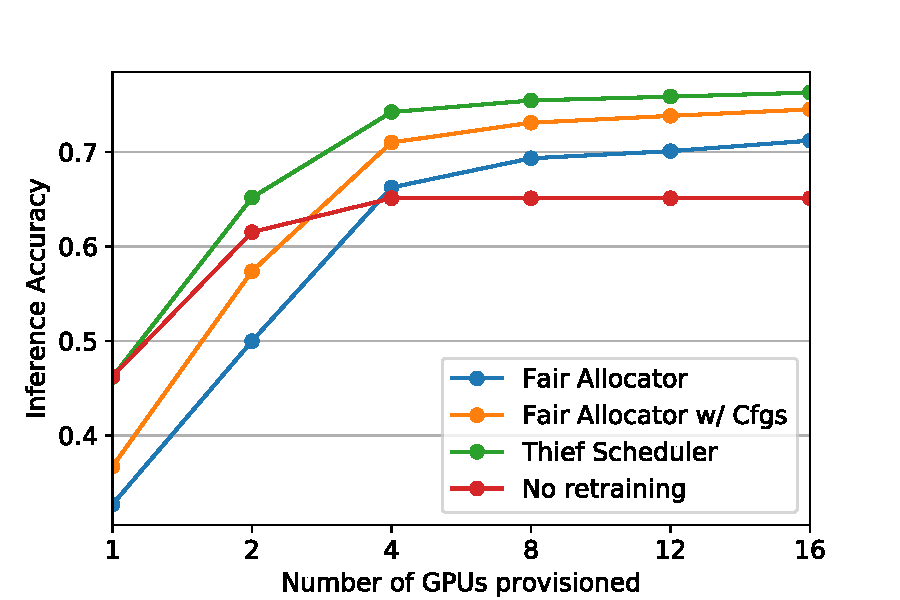
\includegraphics[width=0.4\textwidth]{results/schedcompare_10cams.pdf}
% 	\caption{\small \bf Our performance gain over baselines increases with more GPUs. \romil{Instead of just mean over cameras, consider putting error bars at every marker}}
% 	\label{fig:scalability-gpus}
% \end{figure}



\begin{figure}
  \centering
  \begin{subfigure}[t]{0.5\linewidth}
    \centering
    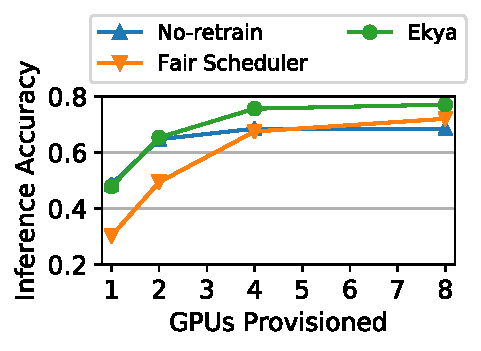
\includegraphics[width=\linewidth]{results/multicam/multicam_acc_vs_res_cityscapes.pdf} 
    \caption{\small Cityscapes}
    \label{fig:scalability-gpus-cityscapes}
  \end{subfigure}
  ~~~
  \begin{subfigure}[t]{0.5\linewidth}
    \centering
    % 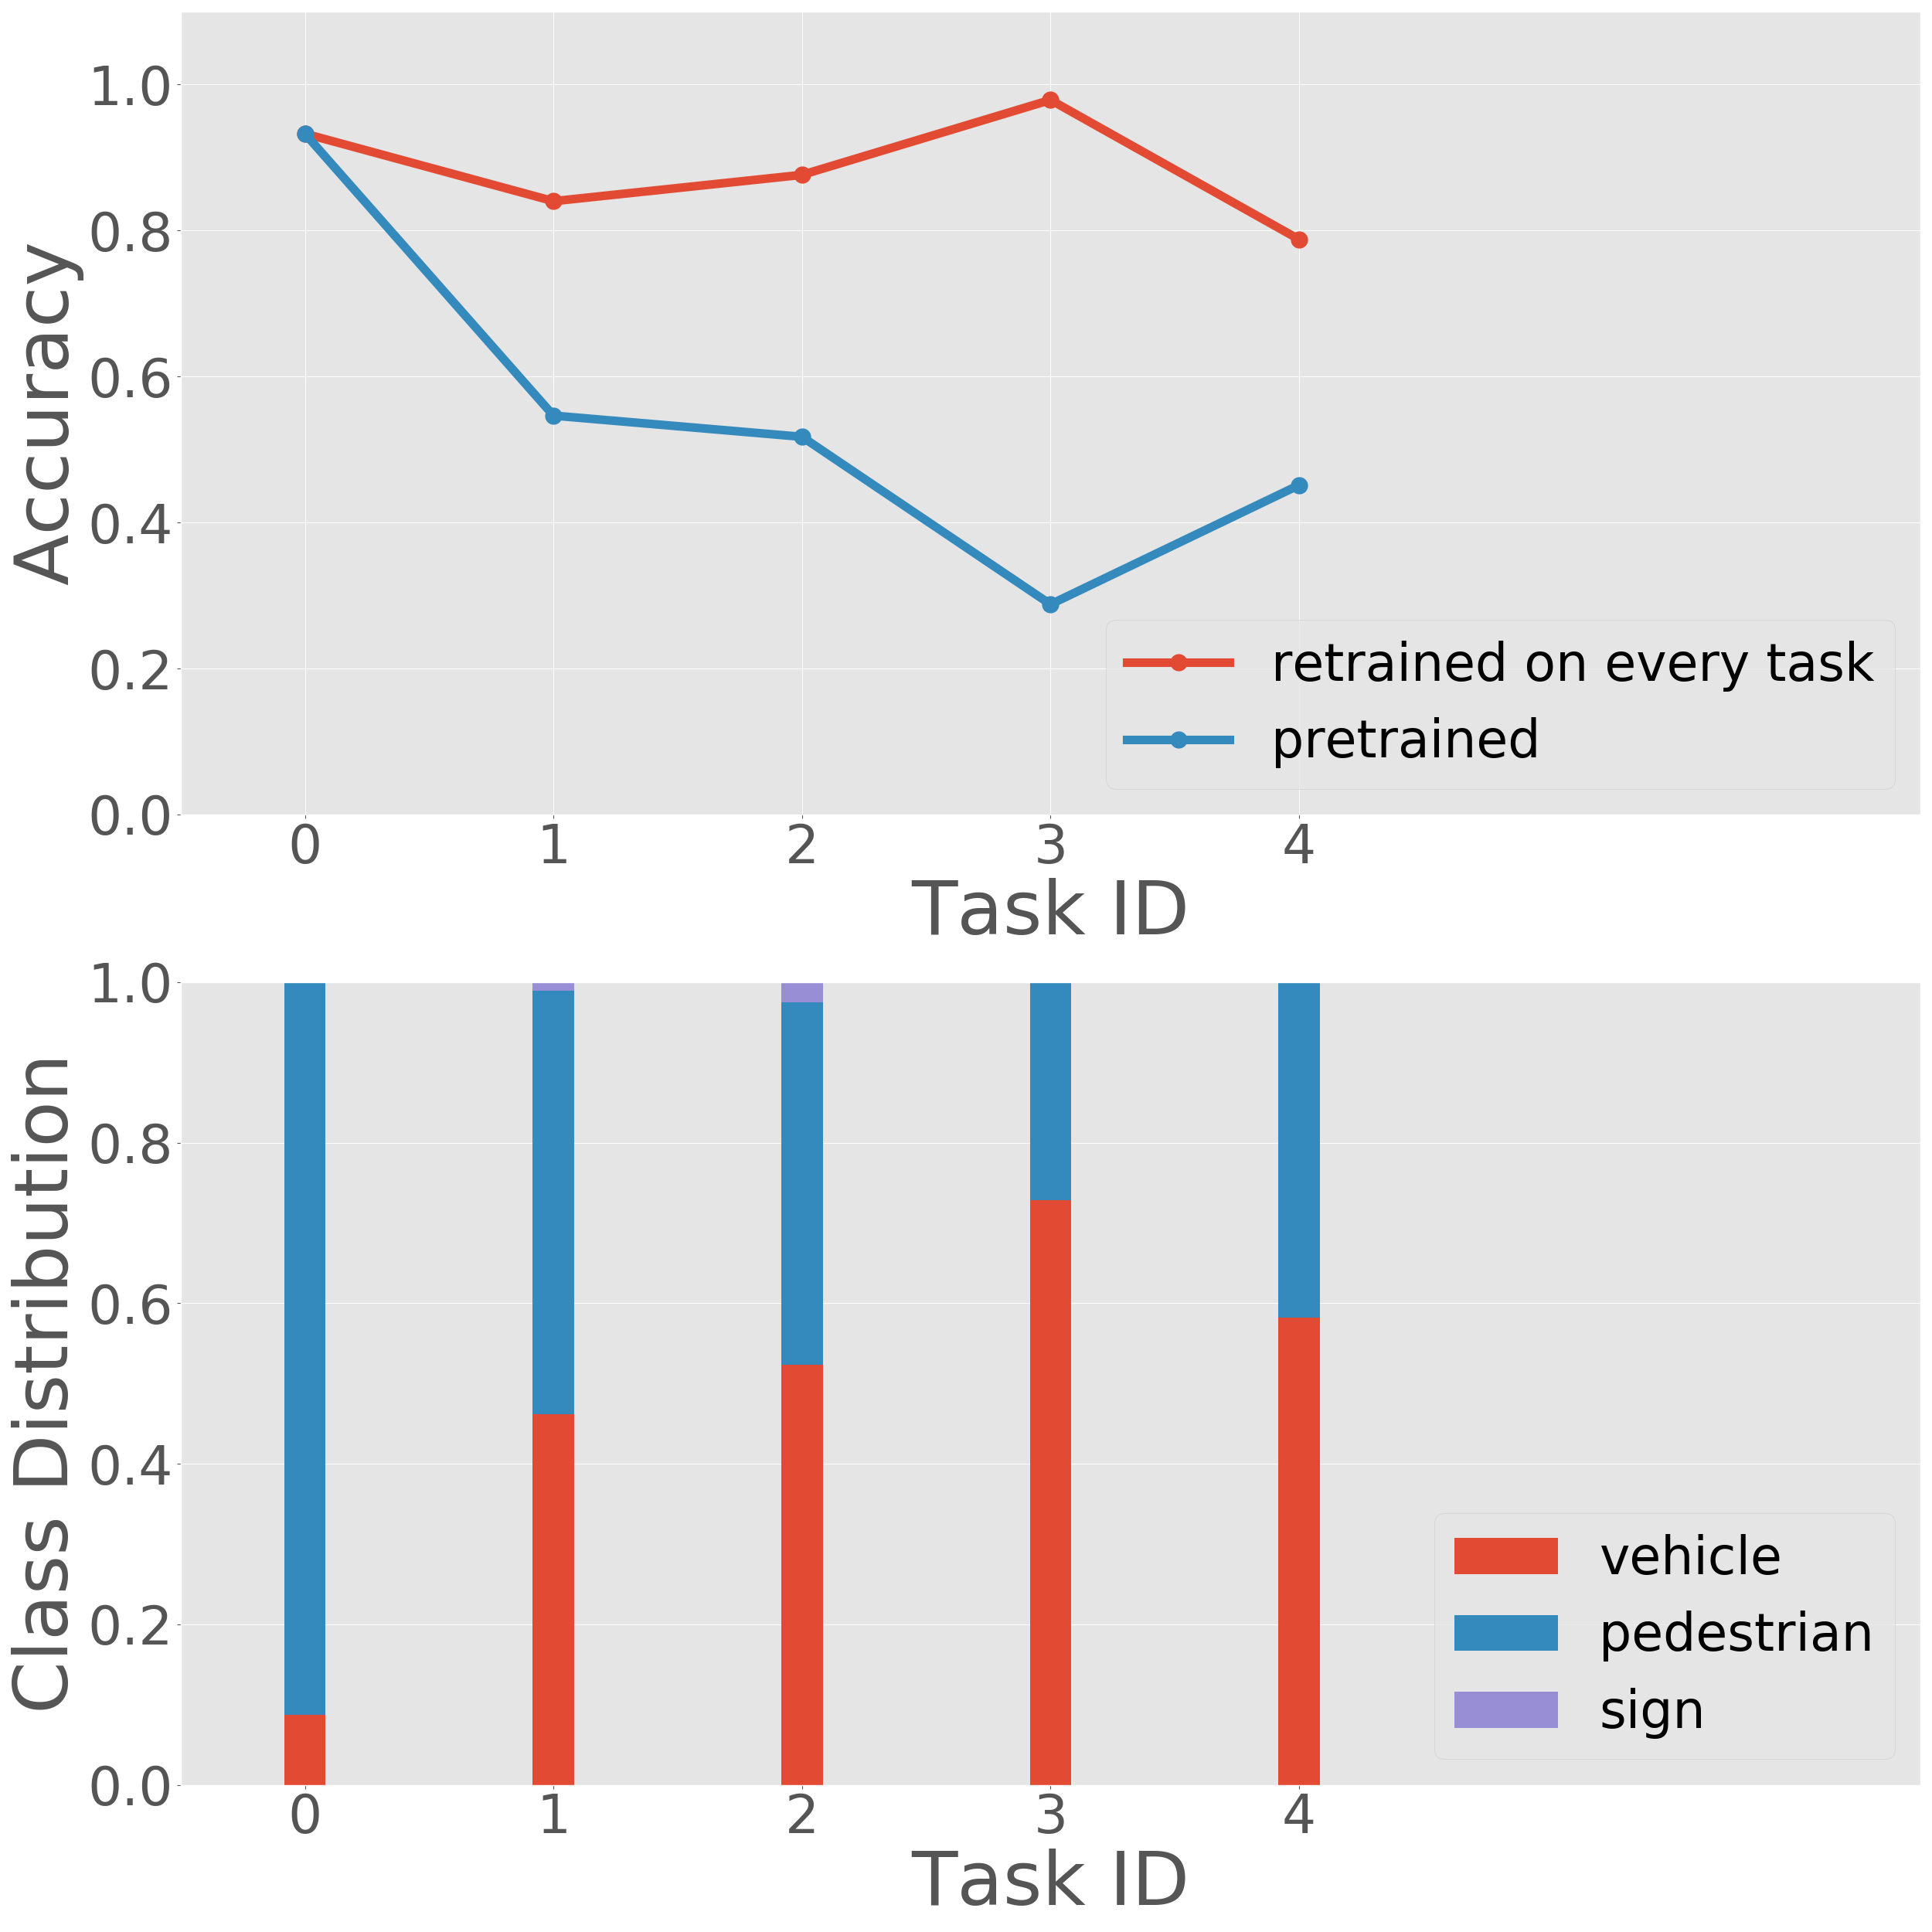
\includegraphics[width=\linewidth]{figures/motivation/Class_Incrementality/class_distribution_change_sf_27.png}
    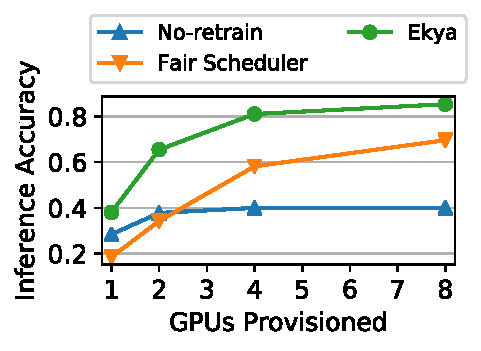
\includegraphics[width=\linewidth]{results/multicam/multicam_acc_vs_res_waymo.pdf}
     \caption{\small Waymo}
    \label{fig:scalability-gpus-waymo}
  \end{subfigure}
  \caption{\small \bf Our performance gain over baselines increases with more GPUs. \romil{Instead of just mean over cameras, consider putting error bars at every marker}}
  \label{fig:scalability-gpus}
\end{figure}

% \begin{figure}
% 	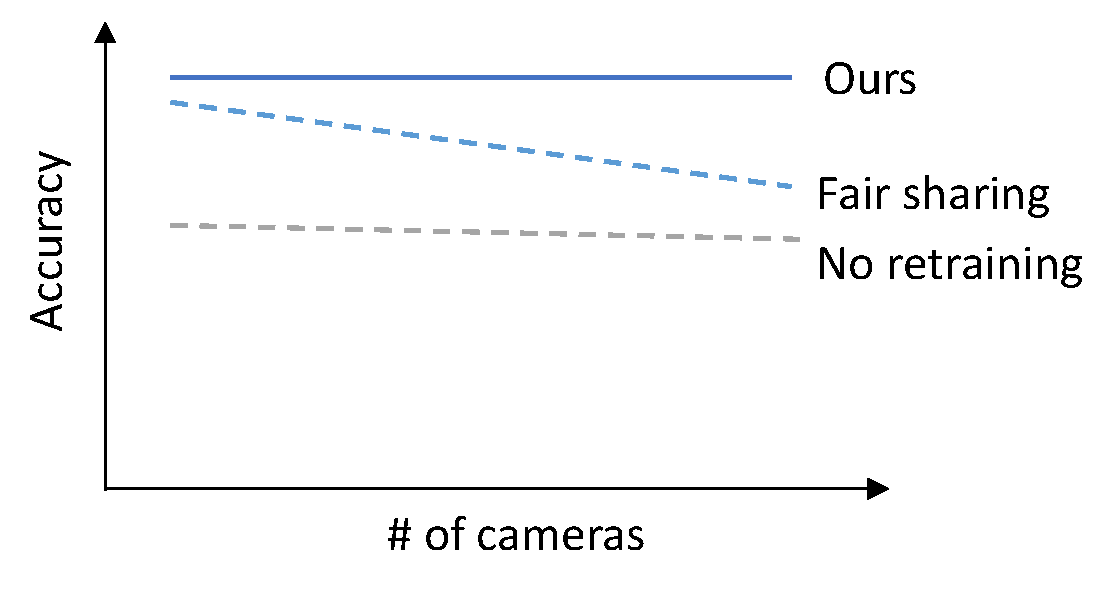
\includegraphics[width=0.4\textwidth]{figures/eval_placeholders/scalability-cameras.pdf}
% 	\caption{\small \bf Our performance gain over baselines increases with more GPUs. \romil{Instead of just mean over cameras, consider putting error bars at every marker}}
% 	\label{fig:scalability-cameras}
% \end{figure}


\begin{figure}
  \centering
  \begin{subfigure}[t]{0.5\linewidth}
    \centering
    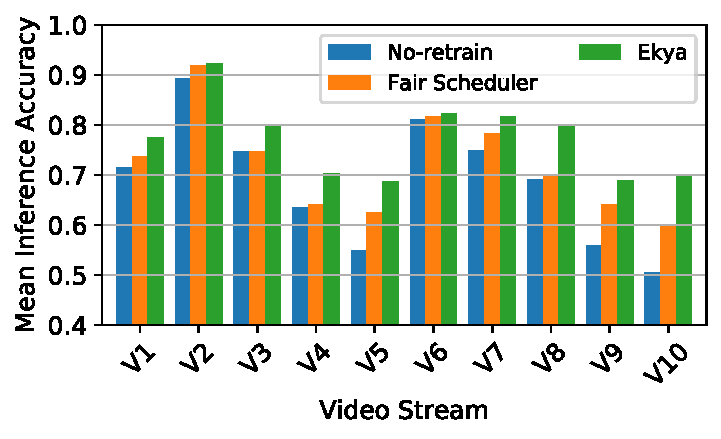
\includegraphics[width=\linewidth]{results/multicam/multicam_individual_stream_acc_cityscapes.pdf} 
    \caption{\small Cityscapes}
    \label{fig:multicam-cities-cityscapes}
  \end{subfigure}
  ~~~
  \begin{subfigure}[t]{0.5\linewidth}
    \centering
    % 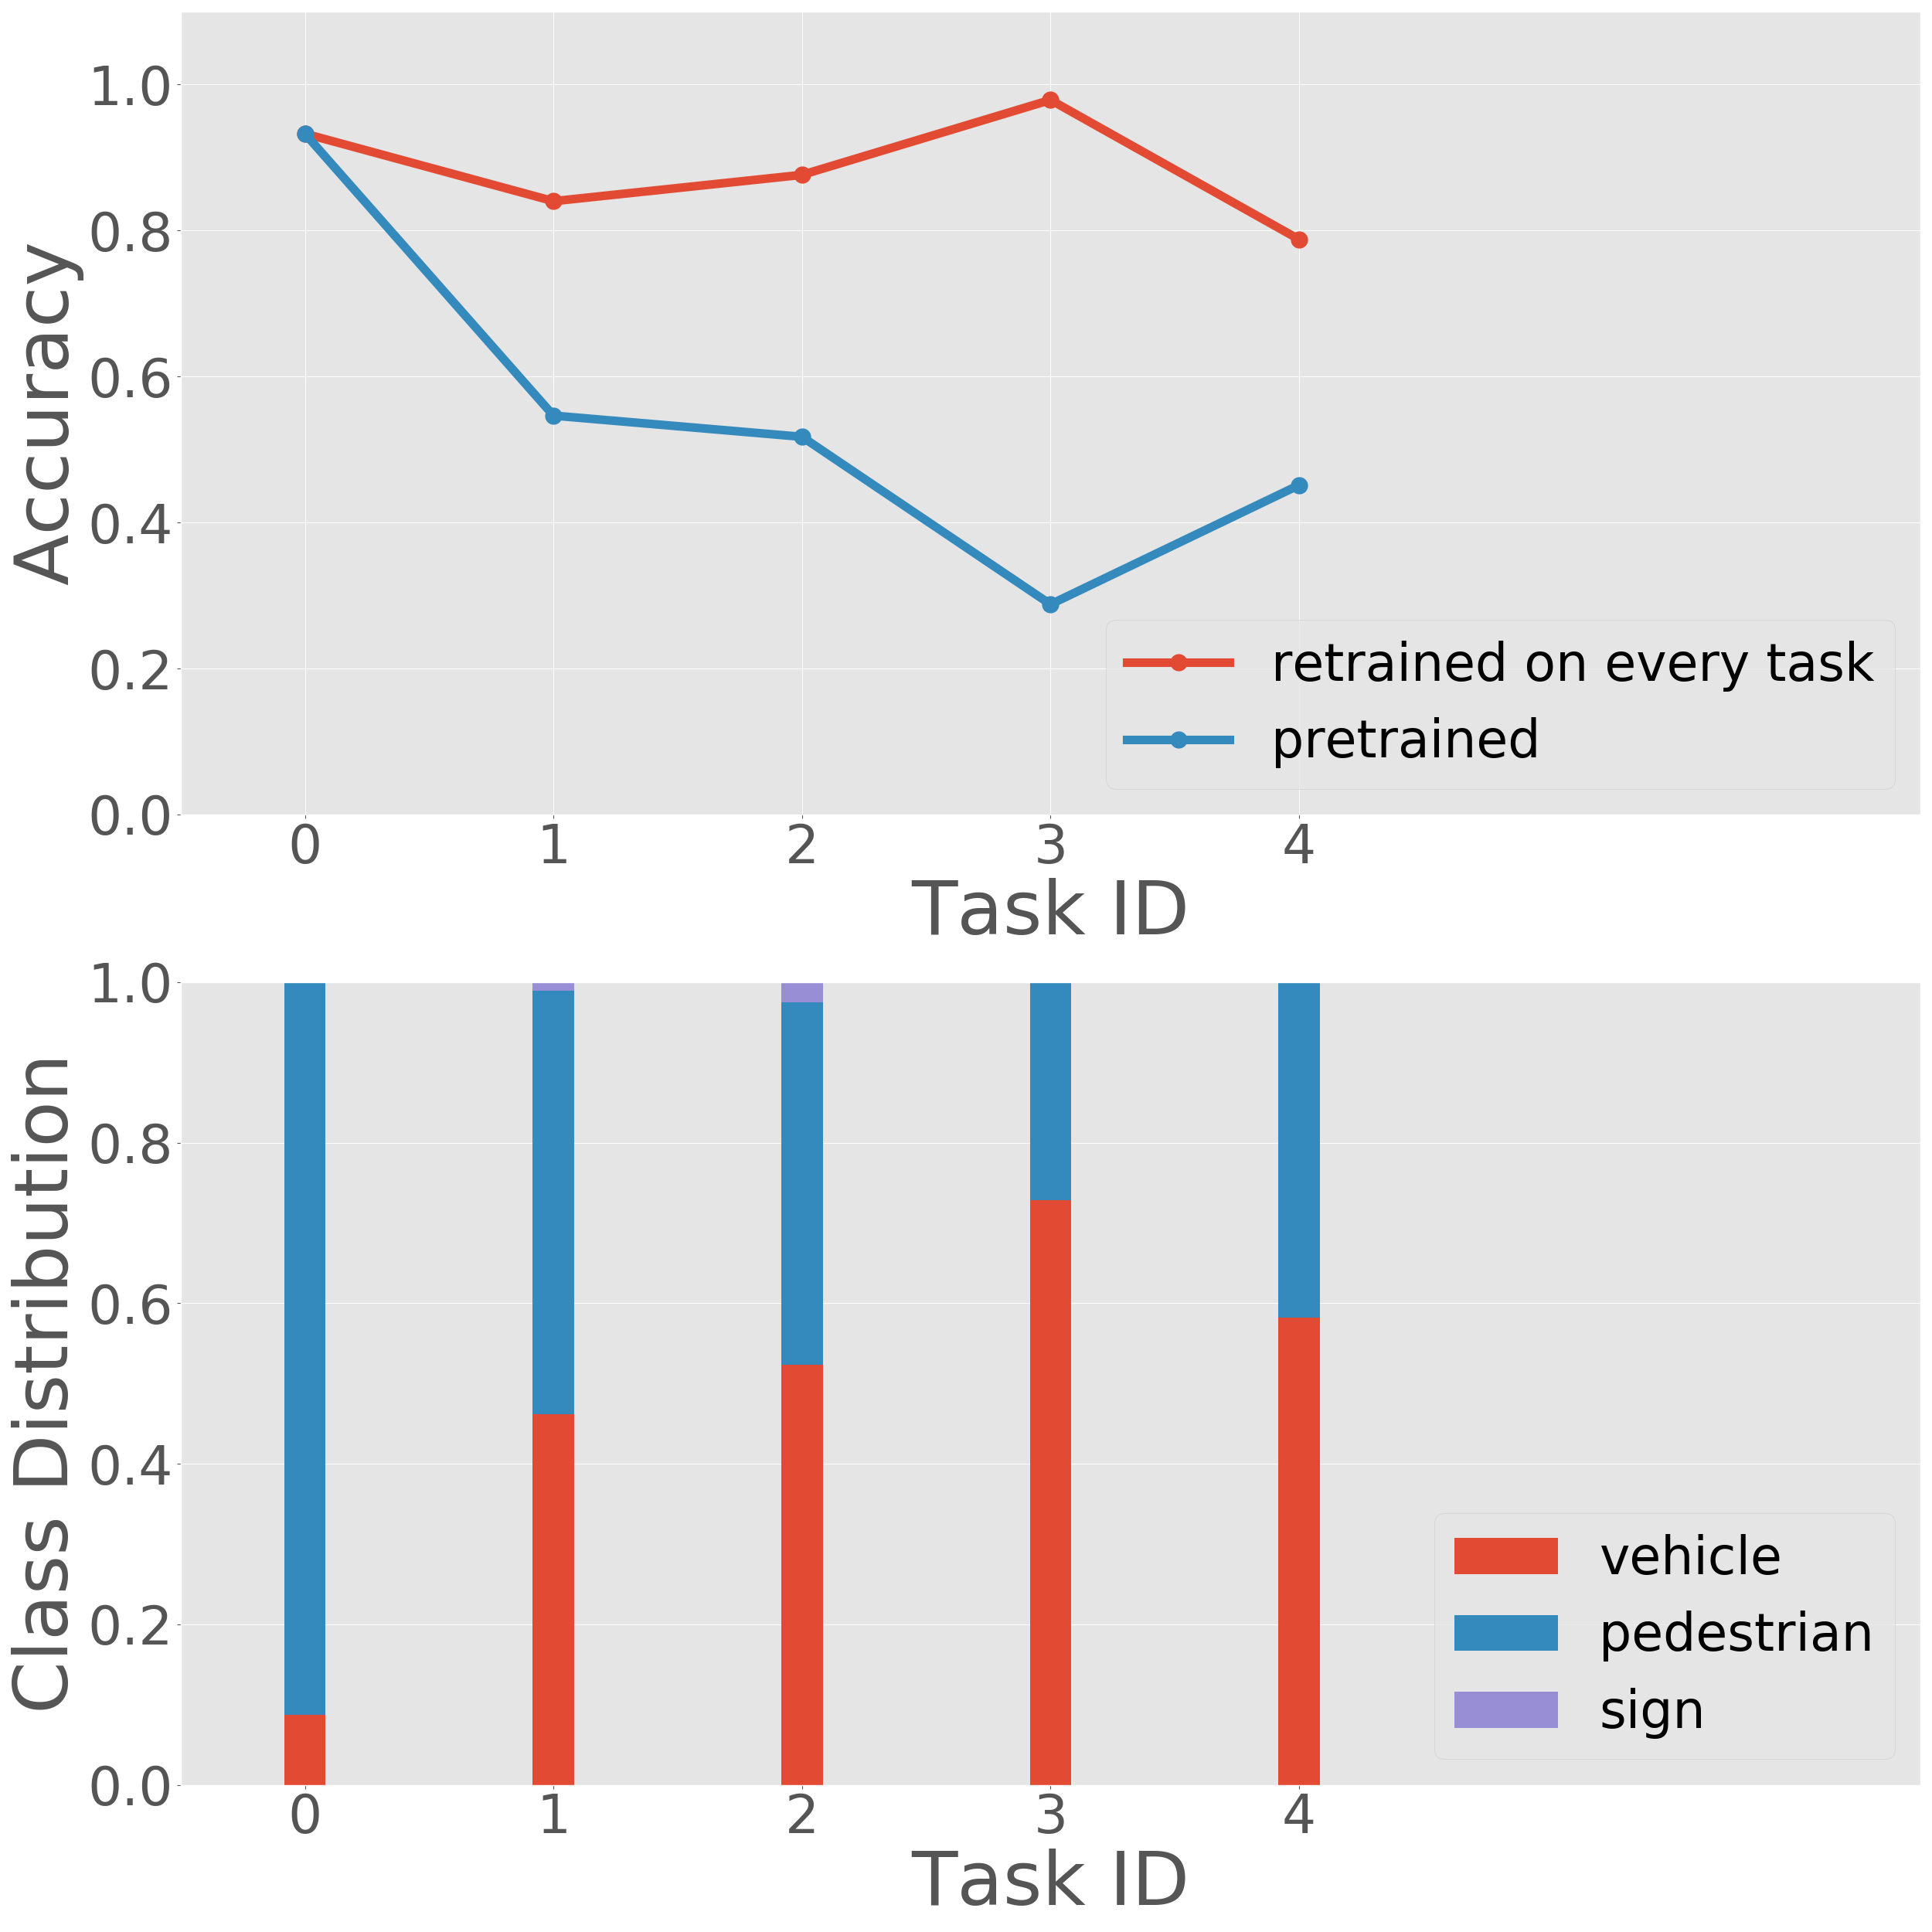
\includegraphics[width=\linewidth]{figures/motivation/Class_Incrementality/class_distribution_change_sf_27.png}
    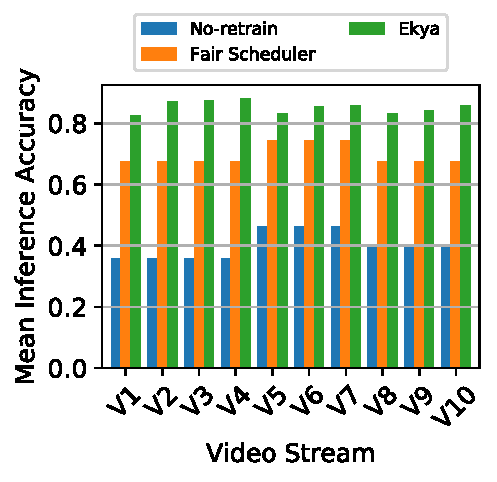
\includegraphics[width=\linewidth]{results/multicam/multicam_individual_stream_acc_waymo.pdf}
     \caption{\small Waymo}
    \label{fig:multicam-cities-waymo}
  \end{subfigure}
  \caption{Multi-video performance: Ours (with continuous retraining) vs. Fair Share Scheduler. Compared across cities, we do consistently better. Some cities see bigger gains, some see smaller.}
  \label{fig:multicam-cities}
\end{figure}

% \begin{figure}[h!]
%  	%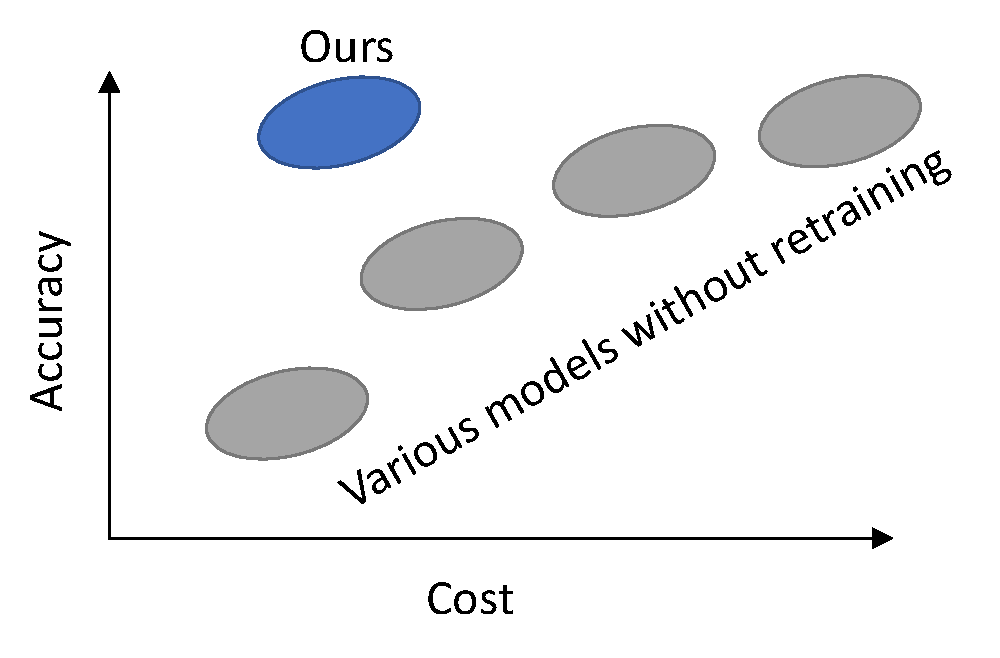
\includegraphics[width=0.4\textwidth]{figures/eval_placeholders/single-tradeoffs.pdf}
%  	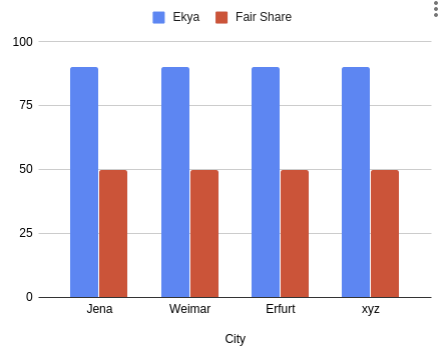
\includegraphics[width=0.4\textwidth]{figures/eval_placeholders/singlecam_e2e.png}
% 	\caption{\small \bf Multi-video performance: Ours (with continuous retraining) vs. Fair Share Scheduler. Compared across cities, we do consistently better. Some cities see bigger gains, some see smaller.}
% 	\label{fig:multi-acrosscities}
% \end{figure}

\begin{figure}
	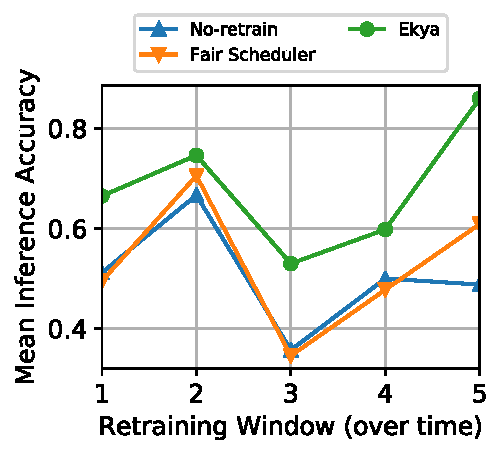
\includegraphics[width=0.4\textwidth]{results/multicam/multicam_taskwise_acc_zurich_4_cityscapes.pdf}
	\caption{\small \bf Timeseries of our performance vs. fair sharing. Again, adaptive resource sharing constantly outperforms fair sharing. \romil{Accuracy drops over time.}}
	\label{fig:multicam-timeseries}
\end{figure}


\begin{table}[]
\begin{tabular}{|c|c|c|c|c|}
\hline
\multirow{2}{*}{\begin{tabular}[c]{@{}c@{}}Video\\ Stream\end{tabular}} & \multirow{2}{*}{Accuracy} & \multicolumn{2}{c|}{GPUs Required} & \multirow{2}{*}{\begin{tabular}[c]{@{}c@{}}Resource\\ Savings\end{tabular}} \\ \cline{3-4}
                                                                        &                           & Ekya        & Fair Scheduler       &                                                                             \\ \hline
V0                                                                      & 76.6\%                    & 4           & 13.4                 & $3.3\times$                                                                 \\ \hline
V1                                                                      & 91.5\%                    & 4           & 4.4                  & $1.1\times$                                                                 \\ \hline
V2                                                                      & 78.1\%                    & 4           & 11.2                 & $2.8\times$                                                                 \\ \hline
V3                                                                      & 68.5\%                    & 4           & 14.9                 & $3.7\times$                                                                 \\ \hline
V4                                                                      & 66.9\%                    & 4           & 17.2                 & $4.3\times$                                                                 \\ \hline
V5                                                                      & 81\%                      & 4           & 6.4                  & $1.6\times$                                                                 \\ \hline
V6                                                                      & 80.9\%                    & 4           & 9.4                  & $2.3\times$                                                                 \\ \hline
V7                                                                      & 76.8\%                    & 4           & 15.1                 & $3.7\times$                                                                 \\ \hline
V8                                                                      & 67.8\%                    & 4           & 14.2                 & $3.5\times$                                                                 \\ \hline
V9                                                                      & 67.9\%                    & 4           & 8.9                  & $2.2\times$                                                                 \\ \hline
\end{tabular}
\label{tab:resource-savings}
\caption{Resource savings for different cities in the cityscapes dataset.}
\end{table}

\subsection{Single video stream performance}
In this section, we evaluate the performance of \name{} on single video stream. In this setup, only one video stream is provided to \name{}, so it must only pick training configurations for one stream and allocate all resources between the training and inference of this stream. 

Figure \ref{fig:single-tradeoffs} highlights the accuracy-cost characteristic demonstrated by different schedulers for 10 video streams from the cityscapes dataset, where each stream is run independently and does not share resources. For a fixed resource cost, \name{} achieves a higher accuracy than both Fair scheduler and no-retrain.  In $V6$, the accuracy gain from retraining is minimal, thus \name{} chooses not to retrain, while the fair scheduler retrains and results in a lower mean inference accuracy.

\begin{figure*}
 	%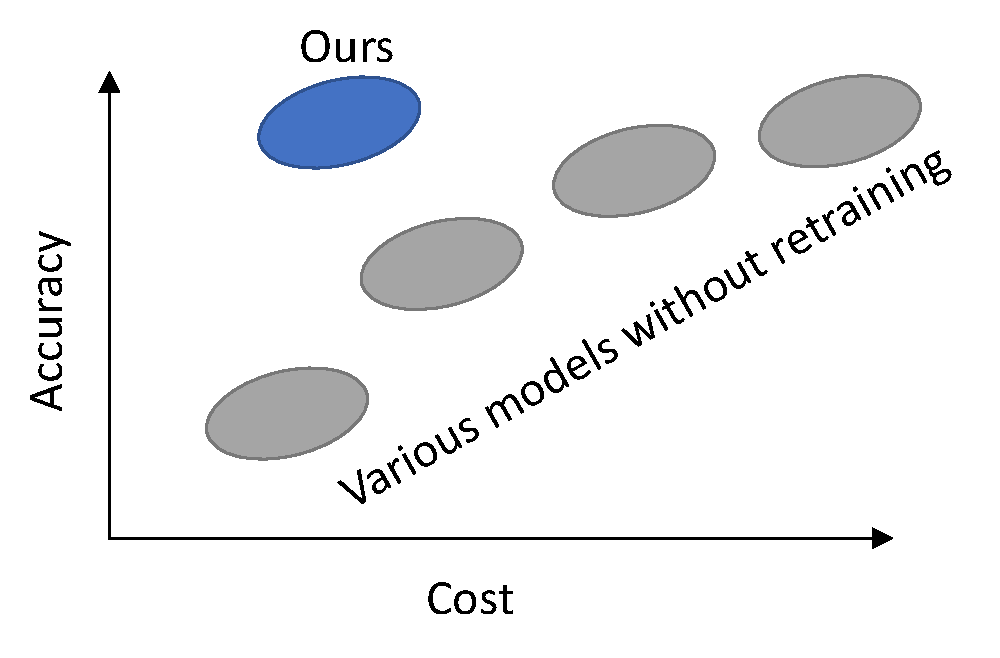
\includegraphics[width=0.4\textwidth]{figures/eval_placeholders/single-tradeoffs.pdf}
 	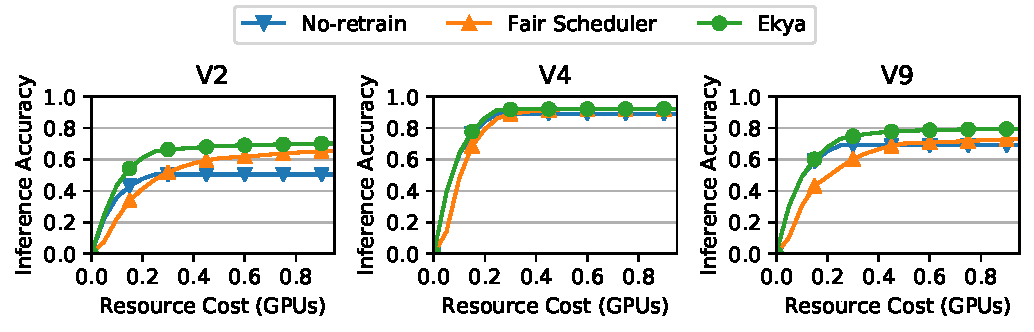
\includegraphics[width=\linewidth]{results/singlecam/singlecam_acc_vs_cost_cityscapes.pdf}
	\caption{\small \bf Single-video performance: Ours (with continuous retraining) vs. various baseline DNN configurations (without retraining). Retraining allows ours to achieve much better accuracy-cost tradeoffs.}
	\label{fig:single-tradeoffs}
\end{figure*}


% \begin{figure}[h!]
% 	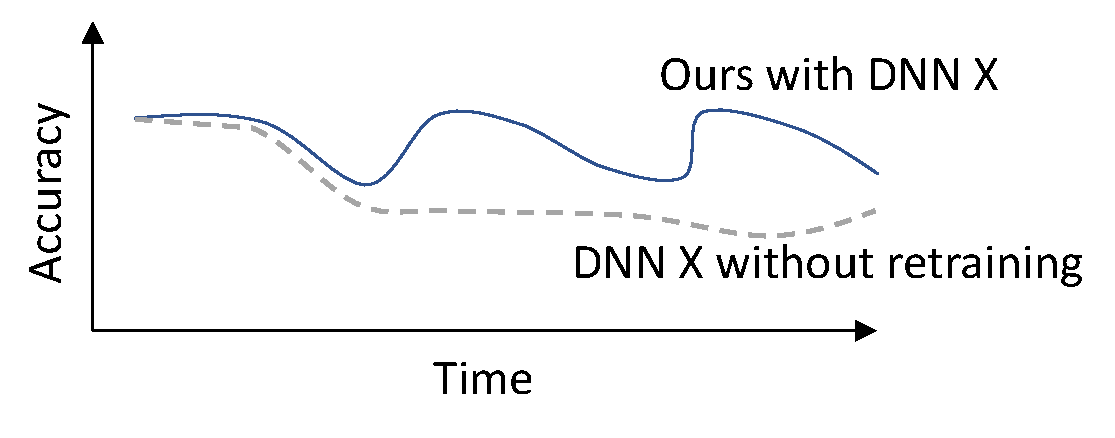
\includegraphics[width=0.4\textwidth]{figures/eval_placeholders/single-timeseries.pdf}
% 	\caption{\small \bf Performance of ours (with continuous retraining) vs. baseline (without retraining) over time. Ours constantly outperforms the baseline due to continuous retraining. \romil{I assume this is similar to Figure 1?}}
% 	\label{fig:single-timeseris}
% \end{figure}


% \begin{figure}[h!]
%  	%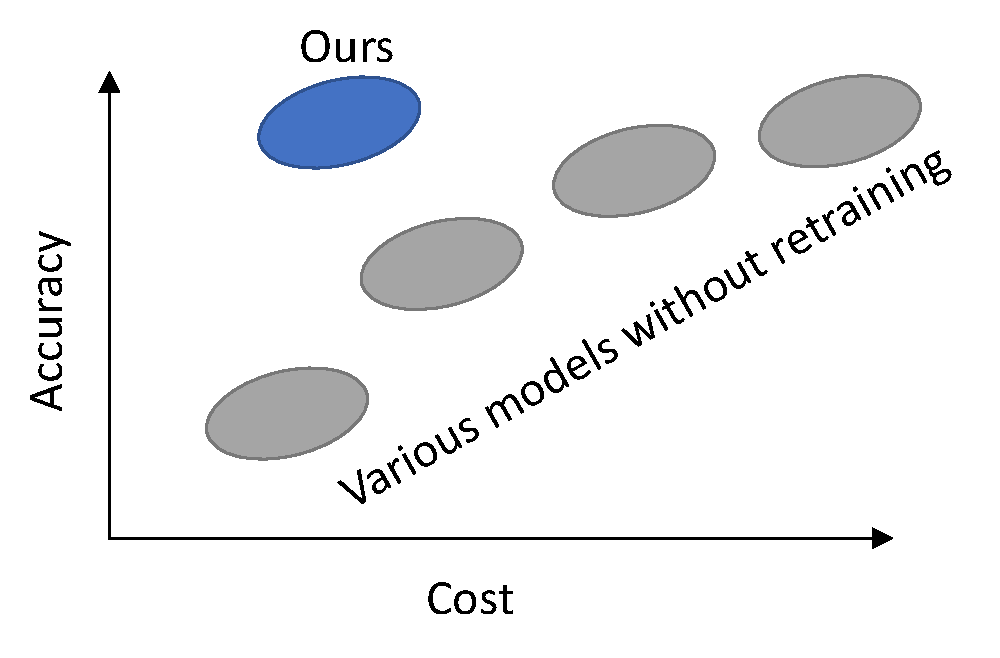
\includegraphics[width=0.4\textwidth]{figures/eval_placeholders/single-tradeoffs.pdf}
%  	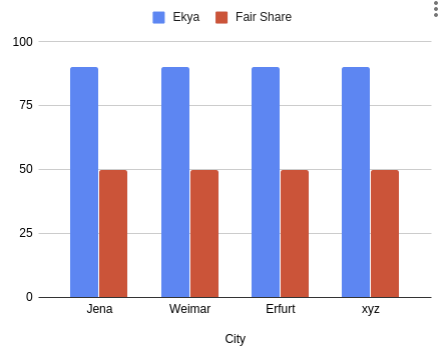
\includegraphics[width=0.4\textwidth]{figures/eval_placeholders/singlecam_e2e.png}
% 	\caption{\small \bf Single-video performance: Ours (with continuous retraining) vs. Fair Share Scheduler. Compared across cities, we do consistently better.}
% 	\label{fig:single-acrosscities}
% \end{figure}

\subsection{Implementation results}

\subsection{Sensitivity analysis}
\begin{itemize}
    \item Sensitivity to $\delta$ resource allocation quantum. \romilc{Affects the speed of convergence}
    \item Sensitivity to errors in profiling \cref{fig:sensitivity-accuracy-error}
    \item Sensitivity to hyperparameter configurations - Remove some of the best hyperparameters. \romilc{Ablation - remove hyperparameters, remove scheudling}
\end{itemize}

\begin{figure}
	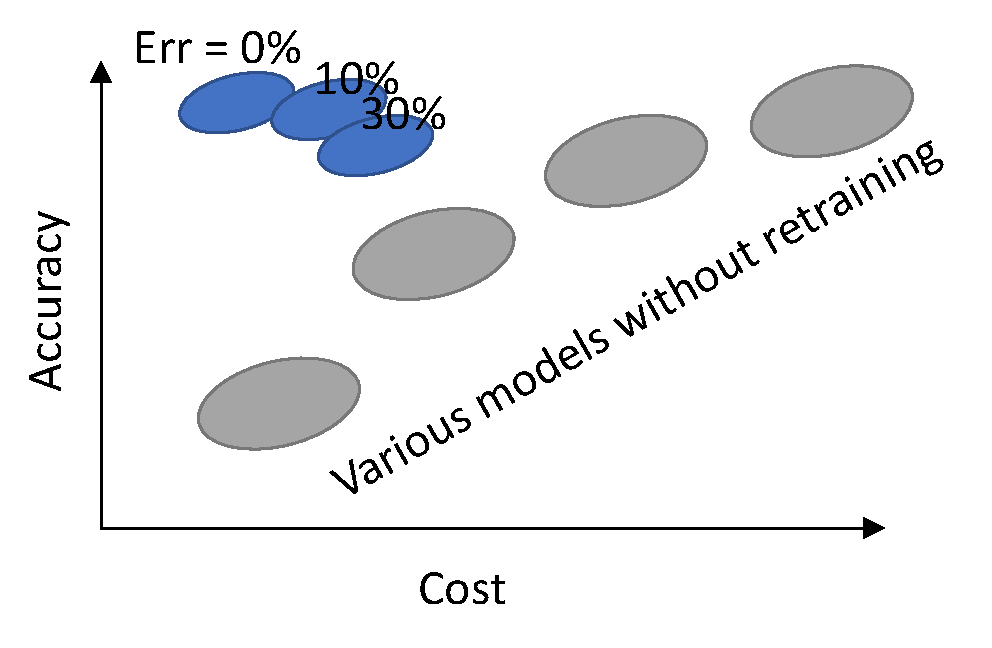
\includegraphics[width=0.4\textwidth]{figures/eval_placeholders/sensitivity-accuracy-error.pdf}
	\caption{\small \bf We add a controlled amount of error to the accuracy prediction and our performance does degrade but only marginally. \romil{Pick 5 cities, horizontal graph}}
	\label{fig:sensitivity-accuracy-error}
\end{figure}


\begin{figure}
  \centering
  \begin{subfigure}[t]{\linewidth}
    \centering
    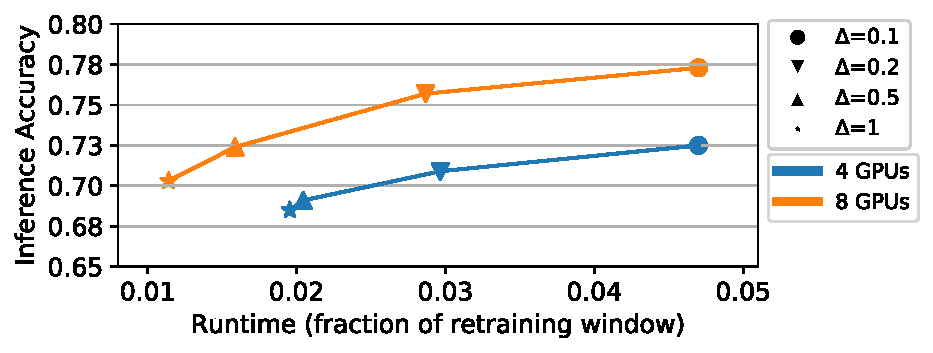
\includegraphics[width=\linewidth]{results/sensitivity/sensitivity_delta_acc_runtime_cityscapes_48gpu.pdf}
  \end{subfigure}
%   \begin{subfigure}[t]{0.5\linewidth}
%     \centering
%     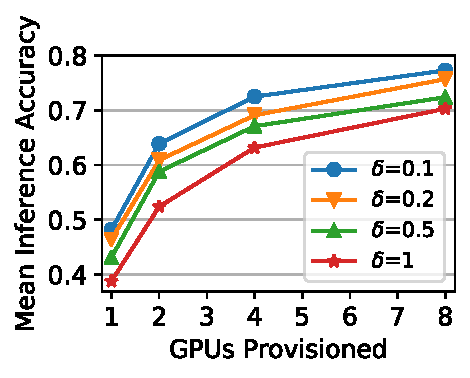
\includegraphics[width=\linewidth]{results/sensitivity/sensitivity_delta_cityscapes.pdf} 
%     \caption{\small Accuracy}
%     \label{fig:scalability-gpus-cityscapes}
%   \end{subfigure}
%   ~~~
%   \begin{subfigure}[t]{0.5\linewidth}
%     \centering
%     % 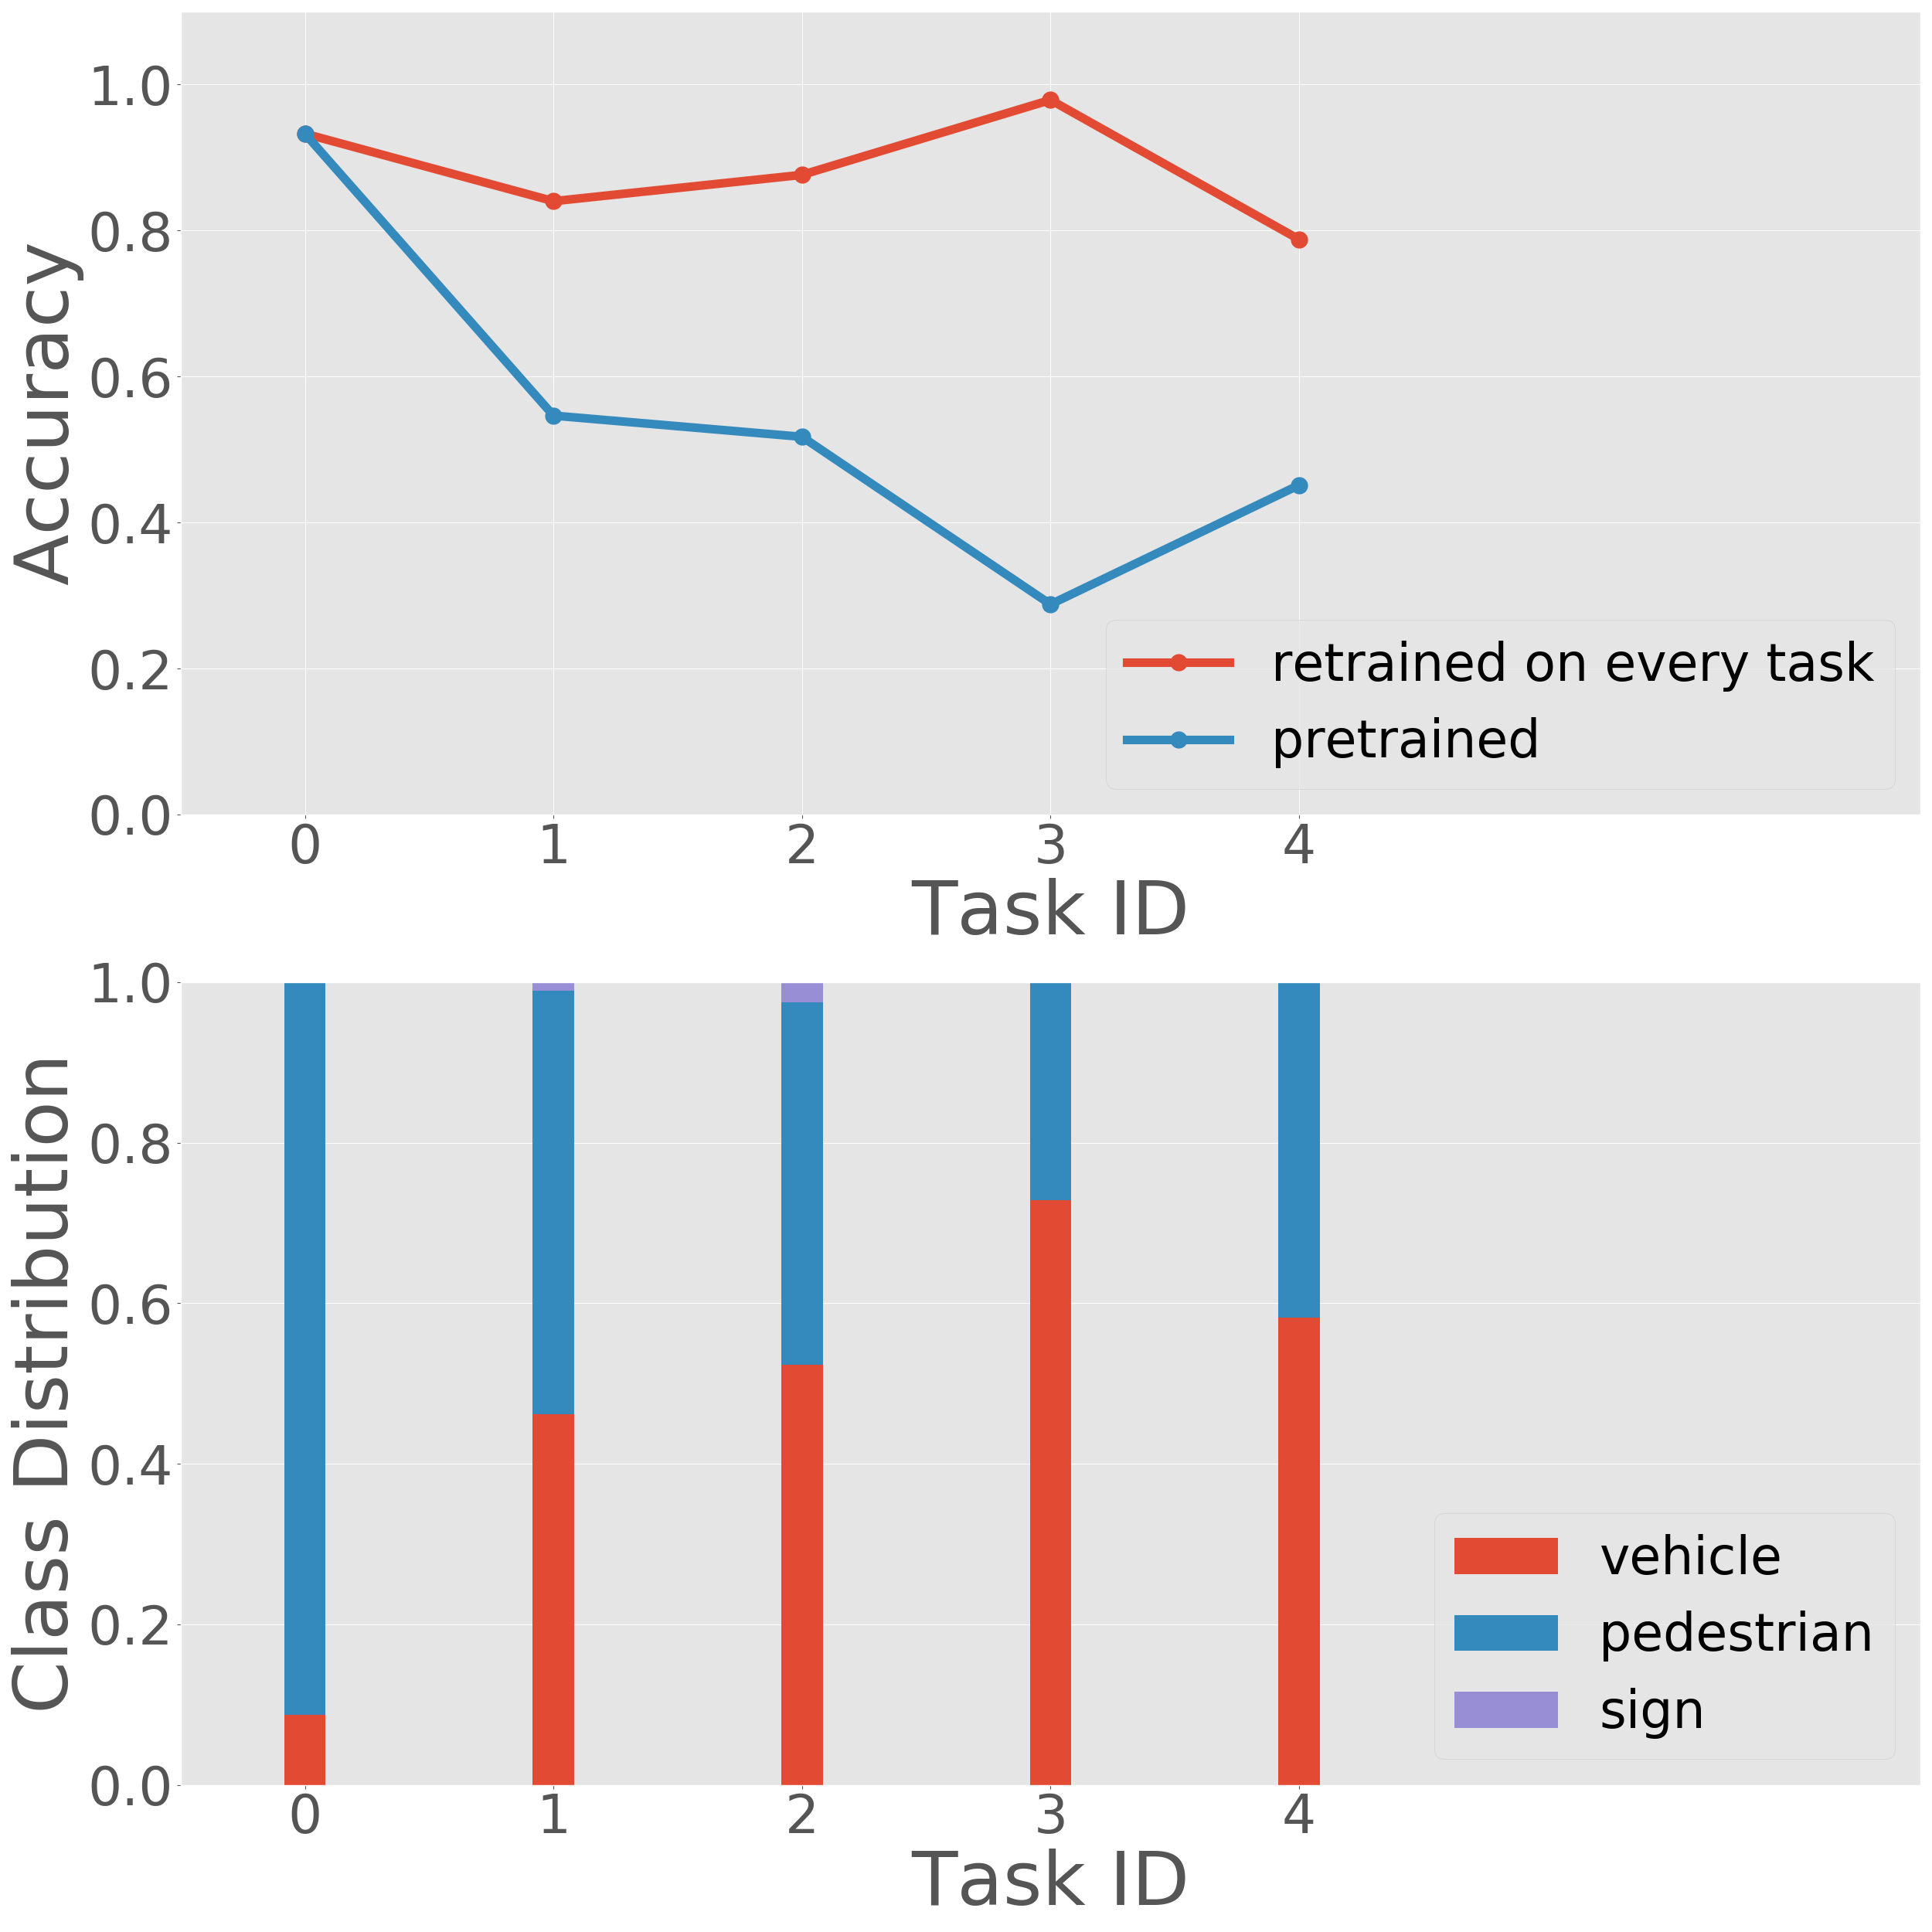
\includegraphics[width=\linewidth]{figures/motivation/Class_Incrementality/class_distribution_change_sf_27.png}
%     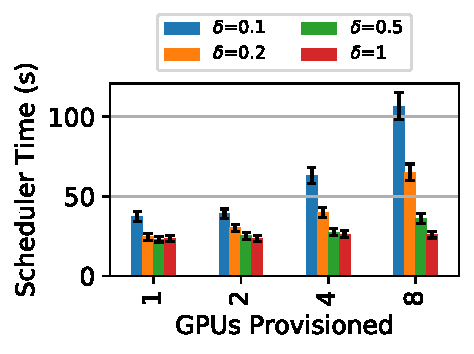
\includegraphics[width=\linewidth]{results/sensitivity/sensitivity_delta_runtime_cityscapes.pdf}
%      \caption{\small Runtime}
%     \label{fig:scalability-gpus-waymo}
%   \end{subfigure}
  \caption{\small \bf Effect of the $\delta$ parameter on the thief scheduler. Larger values decrease the accuracy but are faster to compute.}
  \label{fig:sensitivity-delta}
\end{figure}

% \begin{figure}[h!]
% 	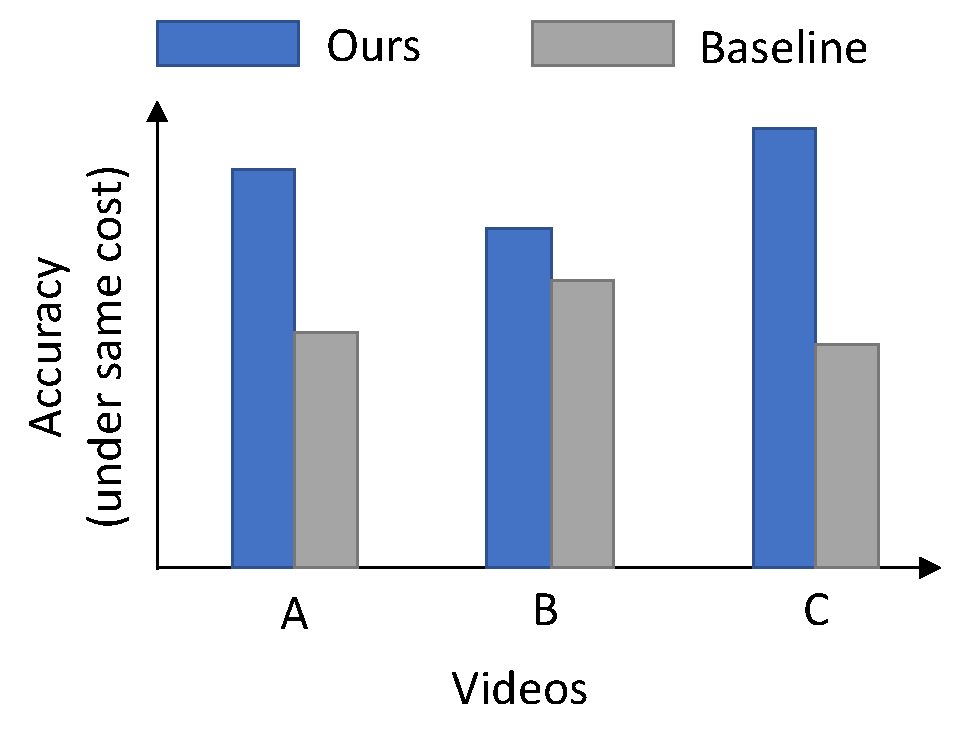
\includegraphics[width=0.4\textwidth]{figures/eval_placeholders/sensitivity-video-accuracy.pdf}
% 	\caption{\small \bf Improvement by videos: Accuracy comparison ours vs baseline on different videos (with given cost budget).}
% 	\label{fig:sensitivity-video-accuracy}
% \end{figure}

\subsection{Alternate design points}

\noindent{\bf Cloud retraining.}

\noindent{\bf Specialized pre-trained models.}